\chapter{Evaluation}

The last chapter presented an implementation of the method to infer time, size and cost bounds.
This chapter evaluates this implementation against other methods.

For this purpose, two different approaches are used.
First, some selected examples are presented that show the benefit of the presented method in contrast to the method of \cite{koat}.
Second, the implementation is evaluated on an example set of programs.
This set of programs is defined and used by comparable tools with the same objective of inferring time bounds for integer programs.

\section{Evaluating Selected Examples}

This section presents two selected examples to compare the results of the new method with the results of the method of \cite{koat}.
This selection is chosen to show the benefits of the new method and is by no means representative.
Nevertheless, it is able to show the potentials of the new method.

The first evaluated example is the motivational program from the introduction in Figure \ref{fig:motivational_example}.

\begin{figure}
  \centering
  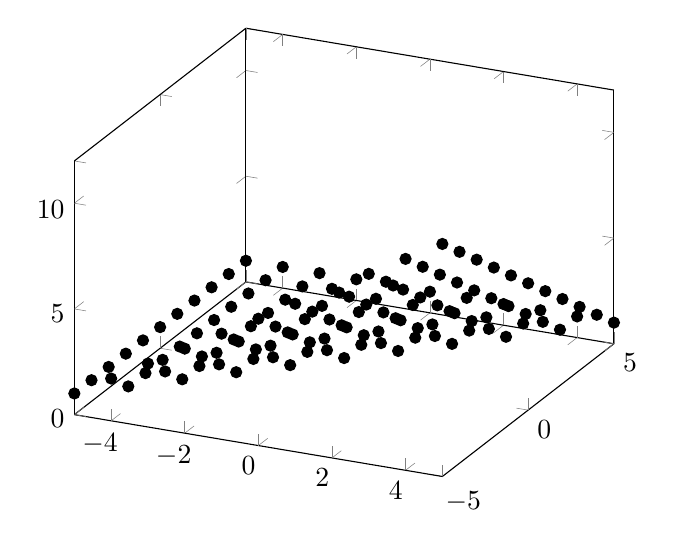
\begin{tikzpicture}
    \begin{axis}
      \addplot3 [
        unbounded coords=jump,
        mesh,
        shader=interp,
        samples at={-5,...,5},
        samples y={11},
        only marks,
      ] {1+max(x-y,0)};
    \end{axis}
  \end{tikzpicture}
  \hfil
  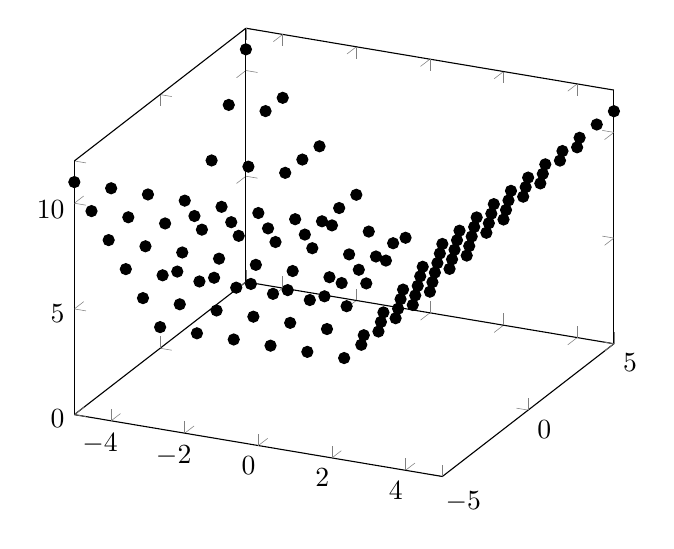
\begin{tikzpicture}
    \begin{axis}
      \addplot3 [
        unbounded coords=jump,
        mesh,
        shader=interp,
        samples at={-5,...,5},
        samples y={11},
        only marks,
      ] {1+abs(max(x,-y))+abs(max(x,-y))};
    \end{axis}
  \end{tikzpicture}
  \caption{Evaluation of the motivational example}
  \label{fig:motivational_evaluation}
\end{figure}


For this program, the new method derives a time complexity of $\maxO{x-y}$, while KoAT \cite{koat} infers a time complexity of $\abs{x}+\abs{y}$.
In the new method, the input state $\valuation_0$ is bounded by two states $\lstate$ and $\ustate$ such that $\lstate \leq \valuation_0 \leq \ustate$ holds.
In the method of KoAT \cite{koat}, the input state $\valuation_0$ is bounded by a single state $m$ such that $-m \leq \valuation_0 \leq m$ holds.
If the states $\lstate$ and $\ustate$ are given, the state $m$ can be defined with $m(v) = \maximum{-\lstate(v),\ustate(v)}$ for each variable $v \in \PVSet$.
Then, it is sufficient to consider the states $\lstate$ and $\ustate$ as parameters for both definitions of time complexity.

Figure \ref{fig:motivational_example} provides two three-dimensional graphs.
The left graph plots the time complexity $\maxO{x-y}$ of the new method and the right graph plots the time complexity $\abs{x}+\abs{y}$ of KoAT \cite{koat}.
We consider input states $\lstate$ and $\ustate$ with $\lstate(v) = \lstate(v')$ and $\ustate(v) = \ustate(v')$ for all variables $v, v' \in \PVSet$.
The graphs show that the time complexities are the same if $-\lstate = \ustate$.
This is the expected result, as $-\lstate = \ustate$ implies that $m = -\lstate = \ustate$.
The new method infers a lower time complexity if the value of $-\lstate$ and $\ustate$ diverges.
The biggest gain is achieved, when $\lstate = \ustate$.
That is if an exact state $\lstate = \valuation_0 = \ustate$ is given as input state for the program.

The second evaluated example is the program presented in the cost bound chapter \ref{fig:cost_ranking_function}.

\begin{figure}
\centering

\begin{tikzpicture}[->,>=stealth',auto,node distance=5cm,
    thick,
    main node/.style={circle,draw,font=\sffamily\Large\bfseries},
    aligned edge/.style={align=left}]

  \node[main node] (0) {$\location_0$};
  \node[main node] (1) [right of=0] {$\location_1$};

  \path[every node/.style={font=\sffamily\small}]
    (0) edge[aligned edge] node[above=0.2cm] {$t_0$} node[below=0.2cm] {$\update = \emph{id}$} (1)
    (1) edge[aligned edge, loop above] node[left=0.2cm] {$t_1$} node[below right=0cm and 0.5cm] {$\update(x) = x - y$\\$\update(y) = y$\\$\guard = \braced{y > 0, x > y}$\\$\cost(t_1)=y$} (1)
    ;
\end{tikzpicture}

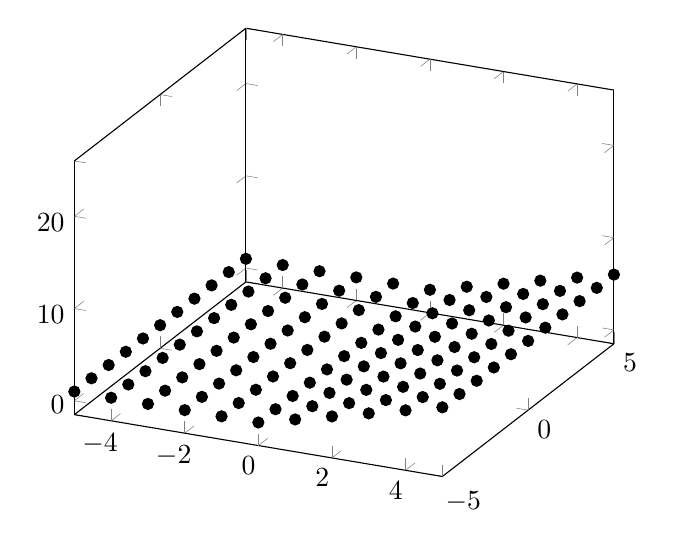
\begin{tikzpicture}
  \begin{axis}[zmax=26]
    \addplot3 [
      unbounded coords=jump,
      mesh,
      shader=interp,
      samples at={-5,...,5},
      samples y={11},
      only marks,
    ] {1+max(x,0)};
  \end{axis}
\end{tikzpicture}
\hfil
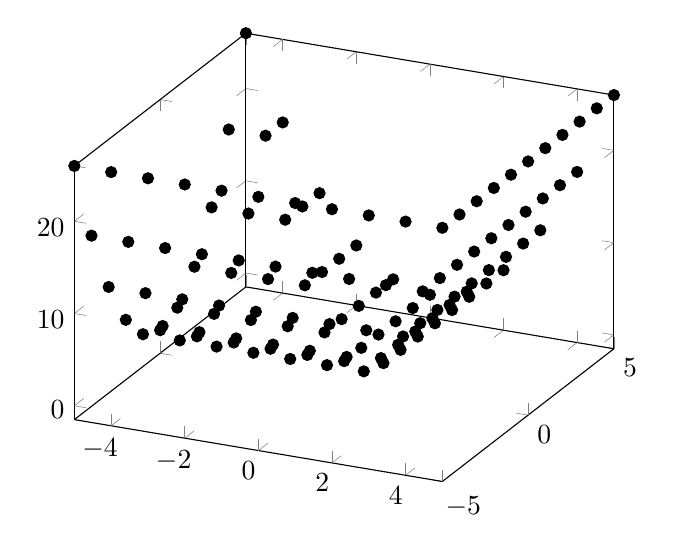
\begin{tikzpicture}
  \begin{axis}[zmax=26]
    \addplot3 [
      unbounded coords=jump,
      mesh,
      shader=interp,
      samples at={-5,...,5},
      samples y={11},
      only marks,
    ] {1+abs(max(x,-y))*abs(max(x,-y))};
  \end{axis}
\end{tikzpicture}

\caption{Evaluation of an example with cost ranking functions yielding a benefit}
\label{fig:cost_ranking_function}
\end{figure}


As already mentioned, the presented method is able to compute a cost bound $\UCost(t_1) = \maxO{x}$ for the transition $t_1$.
Therefore $1 + \maxO{x}$ is a cost bound for the whole program.
Since \cite{koat} does not consider cost ranking functions, its method is only able to compute a cost bound $1 + \abs{x} \cdot \abs{y}$ for the whole program.

The functions are plotted with the same assumptions as the previous example.
The left graph plots the cost complexity $1 + \maxO{x}$ of the new method and the right graph plots the cost complexity $1 + \abs{x} \cdot \abs{y}$ of the method of \cite{koat}.
In this example, the new method yields better results for all input states $\lstate = \ustate$.

\section{Evaluating an Example Set}

This section evaluates the presented implementation on an example set.
This set is a collection of 689 examples introduced by other tools.
We compare the presented method to the results presented in \cite{koat}.
These results include the results of the tool KoAT itself as well as the results of the tools CoFloCo \cite{cofloco1, cofloco2}, Loopus \cite{loopus1, loopus2}, KoAT-TACAS \cite{leike2014ranking}, PUBS \cite{pubs1, pubs2} and Rank \cite{rank}.

For the comparison of the results, it is necessary to project the resulting bounds in $\BoundSet(\PVSet)$ to their asymptotic complexity class.
We use the Big-O-Notation $\landau$ \cite{bigo} to denote the worst-case asymptotic complexity.
We distinguish between constant complexity $\landau(1)$, polynomial complexity of a certain degree $\landau(n^k)$, exponential complexity $\landau(2^n)$ and infinite complexity $\landau(\infty)$.
We use the expected order between these complexity classes (i.e. $\landau(1) \leq \landau(n^k) \leq \landau(2^n) \leq \landau(\infty)$).
The following definition introduces a projection, such that for every bound $b \in \BoundSet(\PVSet)$ the resulting asymptotic complexity $\complexity(b)$ is a valid overapproximation of the actual complexity.

\begin{definition}[Approximation of the Asymptotic Complexity]
  \allowdisplaybreaks
  Let $\VSet$ be a finite set of variables.
  Let $\BoundSet(\VSet)$ be the set of bounds over the variables $\VSet$.
  Then, $\complexity$ is a function which assigns each bound an overapproximation of its asymptotic complexity.
  \begin{align*}
    \complexity(\infty) &= \landau(\infty) \text{ for } \infty \in \BoundSet(\VSet) \\
    \complexity(k) &= \landau(n^0) = \landau(1) \text{ for all } k \in \mathbb{N} \subseteq \BoundSet(\VSet) \\
    \complexity(v) &= \landau(n^1) = \landau(n) \text{ for all } v \in \VSet \subseteq \BoundSet(\VSet) \\
    \complexity(-b) &= \complexity(b) \text{ for all } b \in \BoundSet(\VSet) \\
    \complexity(b_1 + b_2) &= \landau(n^{\maximum{k_1, k_2}}) \text{ for all } b_1, b_2 \in \BoundSet(\VSet) \\
    & \text{ if } \complexity(b_1)=\landau(n^{k_1}) \text{ and } \complexity(b_2)=\landau(n^{k_2}) \\
    \complexity(b_1 + b_2) &= \landau(2^n) \text{ for all } b_1, b_2 \in \BoundSet(\VSet) \\
    & \text{ if } \complexity(b_1)=\landau(2^n) \text{ and } \complexity(b_2)<\landau(\infty) \\
    & \text{ or } \complexity(b_1)<\landau(\infty) \text{ and } \complexity(b_2)=\landau(2^n) \\
    \complexity(b_1 + b_2) &= \landau(\infty) \text{ for all } b_1, b_2 \in \BoundSet(\VSet) \\
    & \text{ if } \complexity(b_1)=\landau(\infty) \text{ or } \complexity(b_2)=\landau(\infty) \\
    \complexity(b_1 \cdot b_2) &= \landau(n^{k_1 + k_2}) \text{ for all } b_1, b_2 \in \BoundSet(\VSet) \\
    & \text{ if } \complexity(b_1)=\landau(n^{k_1}) \text{ and } \complexity(b_2)=\landau(n^{k_2}) \\
    \complexity(b_1 \cdot b_2) &= \landau(2^n) \text{ for all } b_1, b_2 \in \BoundSet(\VSet) \\
    & \text{ if } \complexity(b_1)=\landau(2^n) \text{ and } \complexity(b_2)<\landau(\infty) \\
    & \text{ or } \complexity(b_1)<\landau(\infty) \text{ and } \complexity(b_2)=\landau(2^n) \\
    \complexity(b_1 \cdot b_2) &= \landau(\infty) \text{ for all } b_1, b_2 \in \BoundSet(\VSet) \\
    & \text{ if } \complexity(b_1)=\landau(\infty) \text{ or } \complexity(b_2)=\landau(\infty) \\
    \complexity(\max(b_1, b_2)) &=
    \begin{cases}
      \complexity(b_1) & \text{ if } \complexity(b_1) \geq \complexity(b_2) \\
      \complexity(b_2) & \text{ otherwise }
    \end{cases} \\
    & \text{ for all } b_1, b_2 \in \BoundSet(\VSet) \\
    \complexity(k^b) &=
    \begin{cases}
      \landau(\infty) & \text{ if } \complexity(b)=\landau(\infty) \\
      \landau(2^n) & \text{ otherwise }
    \end{cases} \\
    & \text{ for all } k \in \mathbb{N} \subseteq \BoundSet(\VSet), b \in \BoundSet(\VSet) \\
  \end{align*}
\end{definition}

Note that this definition projects a bound $x-x$ to a complexity $\complexity(x-x) = \landau(n)$.
As already mentioned, the implementation is able to simplify such a bound to an equivalent bound $0$.
Therefore, the better, but still valid complexity $\complexity(0) = \landau(1)$ is determined.
Nevertheless, the implementation is not able to simplify every bound $b$ to an equivalent bound $b'$ with a complexity $\complexity(b')$ better than $complexity(b)$, although such a bound $b'$ may exist.
Such a simplification algorithm has an unreasonable impact on the performance of the implementation.
Therefore, the implemented simplification algorithm does not support the simplification of bounds in general.
It does not consider cases, where it is necessary to analyze multiple levels of operators such as $3 \cdot x^2-(x \cdot x+2 \cdot x^2) = 0$.
Thus, an optimized simplification algorithm might yield better evaluation results without a change to the presented method.

For the parallel execution of the examples, we use the GNU tool 'parallel' \cite{gnuparallel}.
This way, the evaluation of all examples takes \todo{Insert time}{x} seconds with an average of \todo{Insert time}{x} seconds on an Intel i7 processor with four cores.
Therefore, the performance of the new implementation is comparable to other tools of the same domain.

\begin{table}
  \begin{center}
    \label{tab:evaluation}
    \begin{tabular}{l|c|c|c|c|c|c|c|c|c|c|c}
      Method & $\leq\landau(1)$ & $\leq\landau(n)$ & $\leq\landau(n^2)$ & $\leq\landau(n^3)$ & $\leq\landau(n^k)$ & $\leq\landau(2^n)$\\
      \hline
      New method & 113 & 285 & 351 & 358 & 362 & 370 \\
      KoAT       & 131 & 298 & 376 & 383 & 386 & 404 \\
      CoFloCo    & 117 & 270 & 336 & 345 & 347 & 347 \\
      Loopus     & 117 & 247 & 296 & 301 & 306 & 306 \\
      KoAT-TACAS & 118 & 245 & 295 & 295 & 298 & 298 \\
      PUBS       & 109 & 240 & 270 & 278 & 278 & 285 \\
      Rank       & 56  &  72 &  80 &  81 &  81 &  81 \\
    \end{tabular}
  \end{center}
  \caption{Evaluation results}
\end{table}

Table \ref{tab:evaluation} shows the results of the presented implementation compared to the results of the other implementations.
The first column contains the name of the implementation.
The other columns display the number of examples with an inferred asymptotic complexity smaller than the specific asymptotic complexity of the column.
It is assumed that all implementations are sound.
That is, no implementation yields a lower asymptotic complexity than the actual asymptotic complexity of the example.

The reason for the difference between KoAT \cite{koat} and the implementation of the new method is fine-tuning of the established implementation of KoAT \cite{koat}.
For example, KoAT \cite{koat} uses a technique for the chaining of transitions if the current setup does not yield new time bounds.
While chaining is also implemented in the presented implementation, it needs further configuration when it is to apply to yield the same benefits.
Another example is the unrolling of loops which are executed only a constant number of times.
This technique is implemented within KoAT \cite{koat} and might result in a constant time bound where no ranking function is found otherwise.
It can also be implemented within the new method.
Also, the choice of local size bounds and ranking functions leads to a difference in the results.
While a transition $t = (\location, \update, \braced{y=z}, \location')$ with an update $\update$ with $\update(x)=y$ implies two upper local size bounds $\ULSB(t,x)=y$ and $\ULSB(t,x)=z$, the choice among them leads to different result variable graphs and therefore a different setup of SCCs.
Since the size bound method is applied to whole SCCs and a single different result variable in such an SCC might lead to no inferred size bounds, the choice of a local size bound has a huge impact on the size bound method.
The same holds for the choice of ranking functions.
While a ranking function might imply fewer entry transitions than another ranking function, it might nevertheless result in worse time bounds.
That is if there does not exist a time bound for a single entry transition of the former ranking function, while the entry transitions of the latter ranking function are all bounded.
Such considerations can still be implemented within the new method and would then lift the results of the new method to the level of the results of KoAT \cite{koat}.
